\chapter{生体データを用いたコンテンツへの重畳提示システム}

\thispagestyle{myheadings}

 本章では生体データを使いコンテンツに重畳提示する手法について述べる.
図\ref{systemall}に研究の全体像を示す.システムの流れは,コンテンツを視聴しているときの生体データを取得する.
生体データはコンテンツ毎に収集する.集めた生体データから盛り上がっている箇所を推定し抜き出す.
抜き出したデータを基にコンテンツに重畳提示するといった構成である.

\begin{figure}[H]
    \centering
    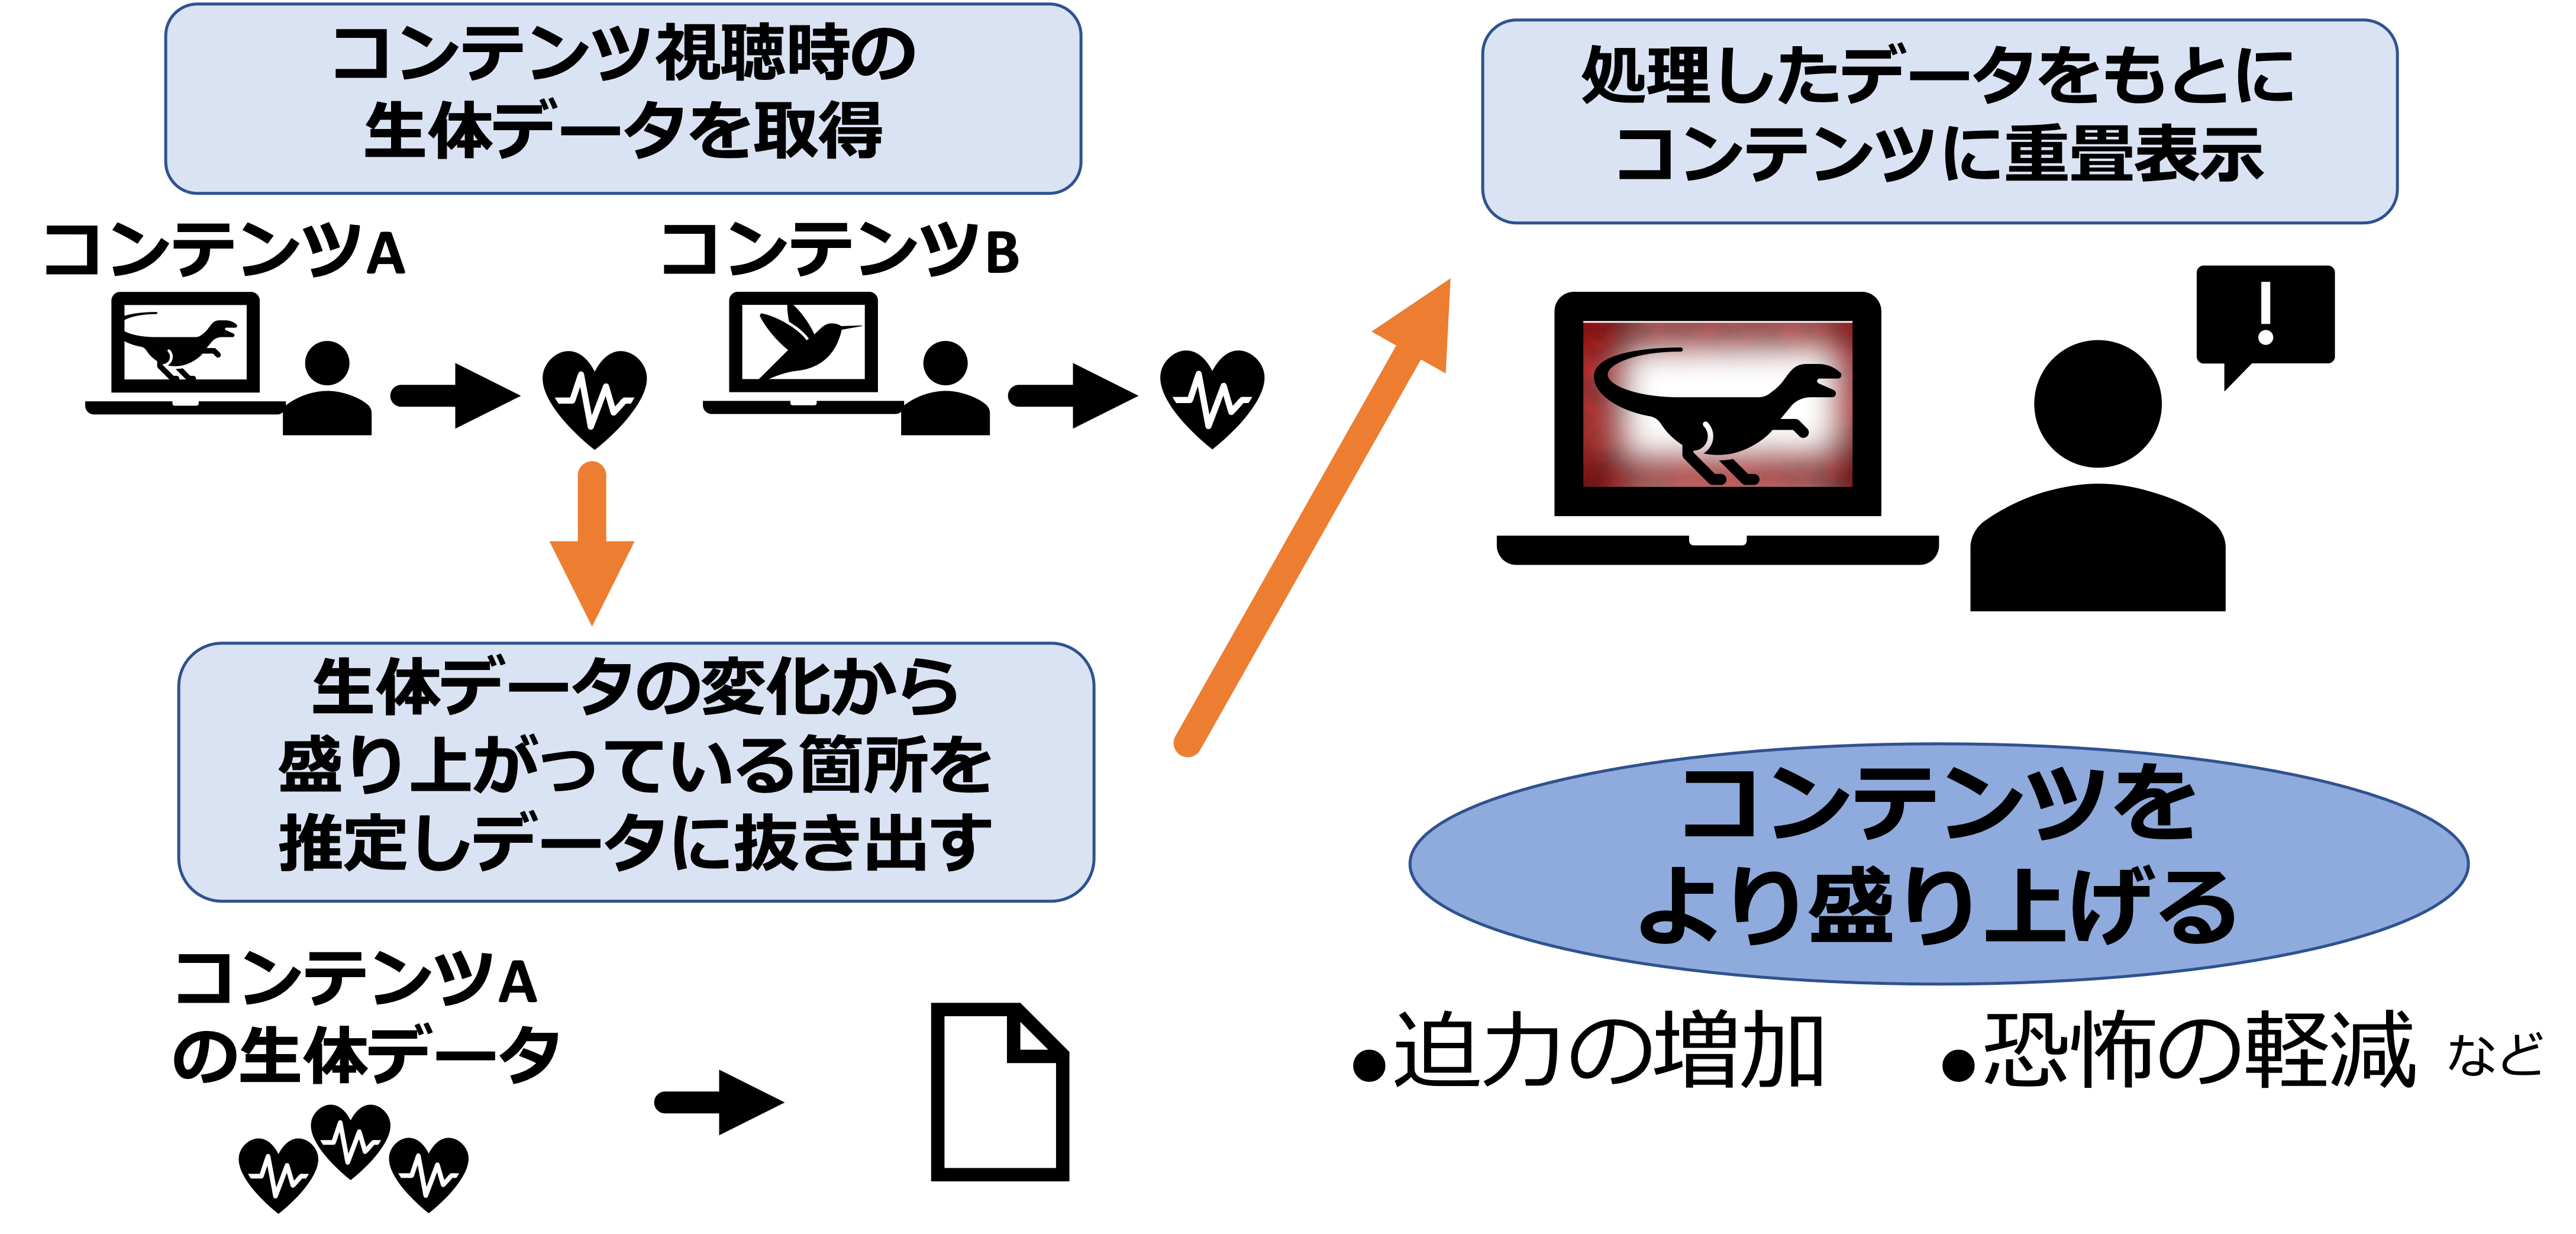
\includegraphics[width=15cm]{images/chapter3/allsysytem.png}
    \caption{システム全体図}
    \label{systemall}
\end{figure}



 コンテンツ視聴時に生体データを取得する理由として,生体データを用いればそのコンテンツに対し視聴者が興奮している箇所を推定可能だからである.
本研究ではコンテンツの盛り上がっている箇所を複数人で共有するため,コンテンツのどの箇所で視聴者が盛り上がっていたのかを生体データを使って推定する.
コンテンツにエフェクトを重畳する目的として生体データを基にコンテンツにエフェクトを重畳することにより,
より盛り上がるコンテンツを楽しむことが可能になるからである.そのため本研究ではコンテンツ視聴時の生体データを取得し,
コンテンツにエフェクトを重畳するシステムにした.
 コンテンツを視聴している時の生体データについて述べる.
収集する生体データとして目の動きに注目したり,額から出る汗の量でコンテンツ視聴時の興奮度を測る方法などが考えられる.
収集する生体データによってコンテンツに対し盛り上がり方を色々な目線で計測するのが可能である.
さまざまな方法で生体データを収集するのができるため,視聴するコンテンツによって適した生体データを取得する.
コンテンツにはYouTubeやNetflixなどのデジタルコンテンツと本や新聞紙などのアナログコンテンツがある.
本研究のシステムではYouTubeなどを視聴している時の生体データの収集だけでなく,新聞紙や本を読んでいる時も盛り上がりポイントを計測するのが可能である.
例として新聞紙を読んでいる時,生体データとして額から出る汗や目の動きなどでは正確に盛り上がるポイントを見つけ出せない.
新聞紙を読んでいる時は心拍数を使い,面白いと感じる記事を読んでいるときの心拍数を計測するなどコンテンツに合わせた生体データを取得する.
またTwitterやInstagram,Facebook,TiktokなどのSNSコンテンツを視聴している時にも使用できる.
 コンテンツへの重畳手法について述べる.コンテンツへの重畳手法としては音を追加したり,画面にエフェクトを表示させる,
デバイスを振動させるなどさまざまである.映画館のような3Dや4DXは映画館の中の決められた映画のみだが,
本研究は生体データを収集すれば自宅でも好きなコンテンツに対し映像体験が可能になる.例として本を読んでいる時の重畳手法は,
徐々に部屋を暗くしたり雑音をはじめの方は流していて盛り上がるポイントが来たら無音にするなど集中しやすい環境に近づけていく.
その他にも音楽を聴いているときはサビにかけてボリュームを上げビートに合わせてデバイスを振動させライブ会場のようなワクワクが体験できたり,
スマートフォンで車のレースゲームをしている時には風を送りゲームに没入感を加える.

\section{本研究のシステム構成}
 本研究で採用したシステムについて述べる.本研究では生体データの収集方法としてスマートウォッチを採用した.
理由として近年スマートウォッチは普及しており,誰でも気軽に生体データを取得できるからである図\ref{watchfukyuu}.今回スマートウォッチはTicWatchE3を使用した図\ref{watche3}.
コンテンツは映画を視聴することにした.コロナ禍により自宅で映画を視聴する機会が増えたためである.
また,映画は盛り上がるポイントが明確に出てくると予想したからである.スマートウォッチを使い映画を視聴している時の生体データとして,心拍数を計測する.
心拍数を計測する理由として,スマートウォッチを使い気軽に計測ができるためである.
また映画を視聴している時は心拍数が頻繁に変化し生体データとして適していると考えたからである.
収集した心拍データは生体データを管理するサーバにアップロードされる.映画には画面に直接エフェクトを重畳する.
映画画面に直接枠を囲うようなエフェクトを表示することで迫力や恐怖などを体験できると考えたからである.
本研究の流れは映画を見ている時の心拍数をスマートウォッチを使って計測し,取得した心拍データをスマートウォッチからサーバにアップロード,
アップロードされた心拍データから心拍数が上昇している箇所のみのデータにする.
その心拍上昇箇所のみの心拍データを基に映画画面に直接画面を囲うようなエフェクトを重畳するという流れになっている.
映画を視聴する時にスマートウォッチを腕に取り付け,スマートウォッチを使い心拍数を計測する.
取得した心拍データはサーバにアップロードされ,心拍数が上昇している箇所だけのデータに抽出処理が行われる.
映画毎に複数人のデータが一つのエフェクト表示に適したデータへと変換される.そのデータを基に映画画面に直接エフェクトが表示されるシステムである.


\begin{figure}[H]
    \centering
    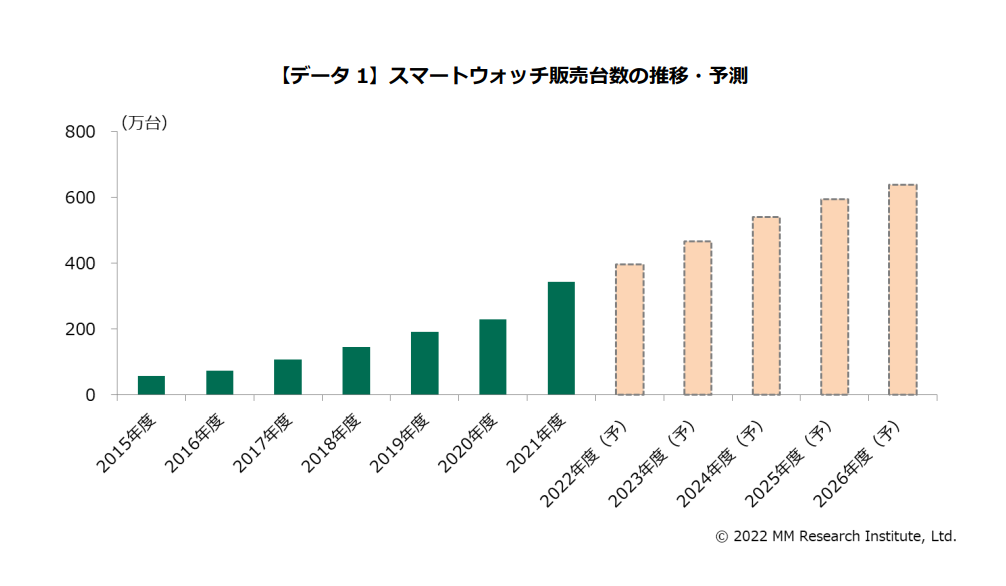
\includegraphics[width=14cm]{images/chapter3/watchreserch.png}
    \caption{スマートウォッチの普及率}
    \label{watchfukyuu}
\end{figure}

\begin{figure}[H]
    \centering
    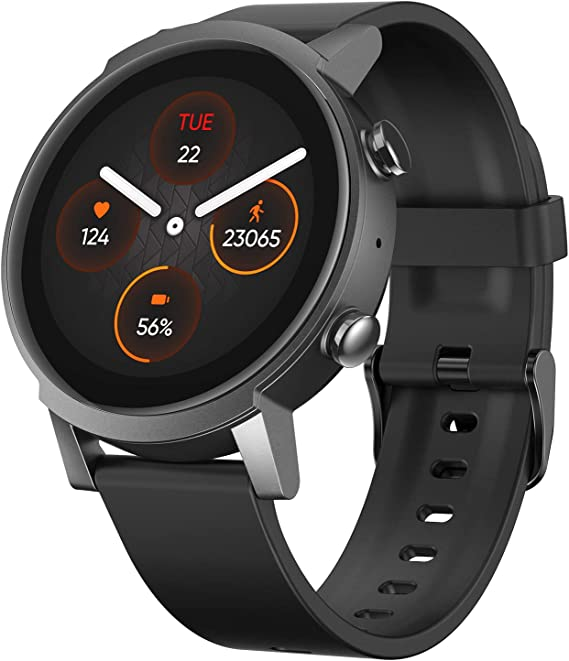
\includegraphics[width=5cm]{images/chapter3/watch.jpg}
    \caption{利用したスマートウォッチ,TicWatchE3}
    \label{watche3}
\end{figure}


\section{心拍データについて}

 本節ではシステムを構成する機能のうち,スマートウォッチを使い心拍データを取得する方法,
収集した心拍データから心拍数が上昇している箇所の抽出方法について述べる.

\subsection{心拍データの収集方法}

 スマートウォッチを使い心拍数を計測する方法を述べる.本研究では映画を視聴している時の心拍数を計測するため,
AndroidStudioで心拍数が取得できるアプリを作成した。アプリ画面を図\ref{bpmget}に示す.
センサ取得ボタンを押すことによって腕につけた時の心拍数を心拍という文字の下に表示できる.
csv file nameに保存したいファイル名を記入し記録開始ボタンを押すことで心拍数の記録が始まる.
心拍数を取得中の画面を図に示す.心拍数の計測が終了したらCSV出力のボタンを押し計測を終了する.
取得した心拍データはCSVファイルとなり生体データを管理するサーバへとアップロードされる.

\begin{figure}[tbh]
    \centering
    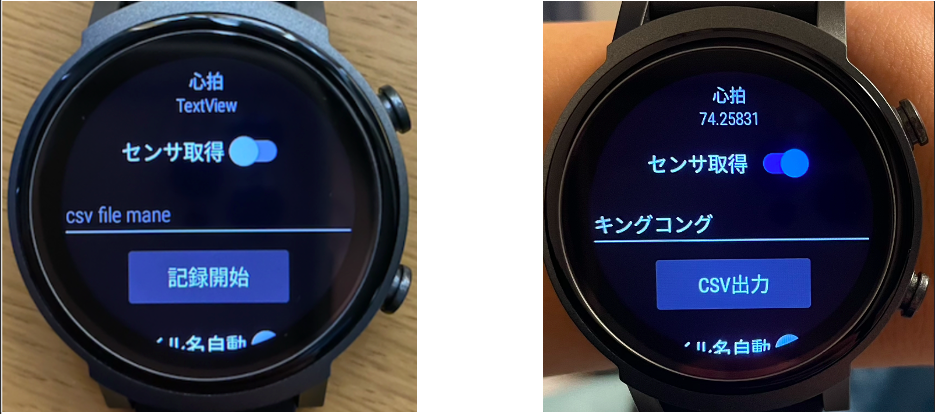
\includegraphics[width=15cm]{images/chapter3/watchgazou.png}
    \caption{心拍数取得画面}
    \label{bpmget}
\end{figure}


\subsection{心拍データの観察}

収集した心拍データを観察する.実際に集めた心拍データの一部をグラフにしたものを表示する図.
映画は「キングコング 髑髏島の巨神」を視聴した人のデータである.集めたデータを観察したところ,人により心拍数の変動が様々であった.
図\ref{hitorime}のように盛り上がりを見せるシーンのみ心拍数が上昇しそれ以外は比較的落ち着いている人がいたが,
図\ref{futarime}のように常に心拍数が上昇と下降を繰り返しており盛り上がっている箇所が把握できない人や、図\ref{sannninme}のように盛り上がりを見せるシーンでは心拍数が大幅に上昇し、
それ以外は上昇と下降を繰り返している人もいた.また人によって映画視聴中の平均心拍数にばらつきがあった.
映画の盛り上がるシーンと心拍数の関係を比較したところ,盛り上がりを見せるシーンで心拍数が上昇している人がいた.
図と図は数分の差はあったものの盛り上がるシーンで平均の心拍数よりも上昇していた.
これより人によって差はあるが映画を視聴している時の盛り上がるシーンでは心拍数が上昇することがわかった.

\begin{figure}[H]
    \centering
    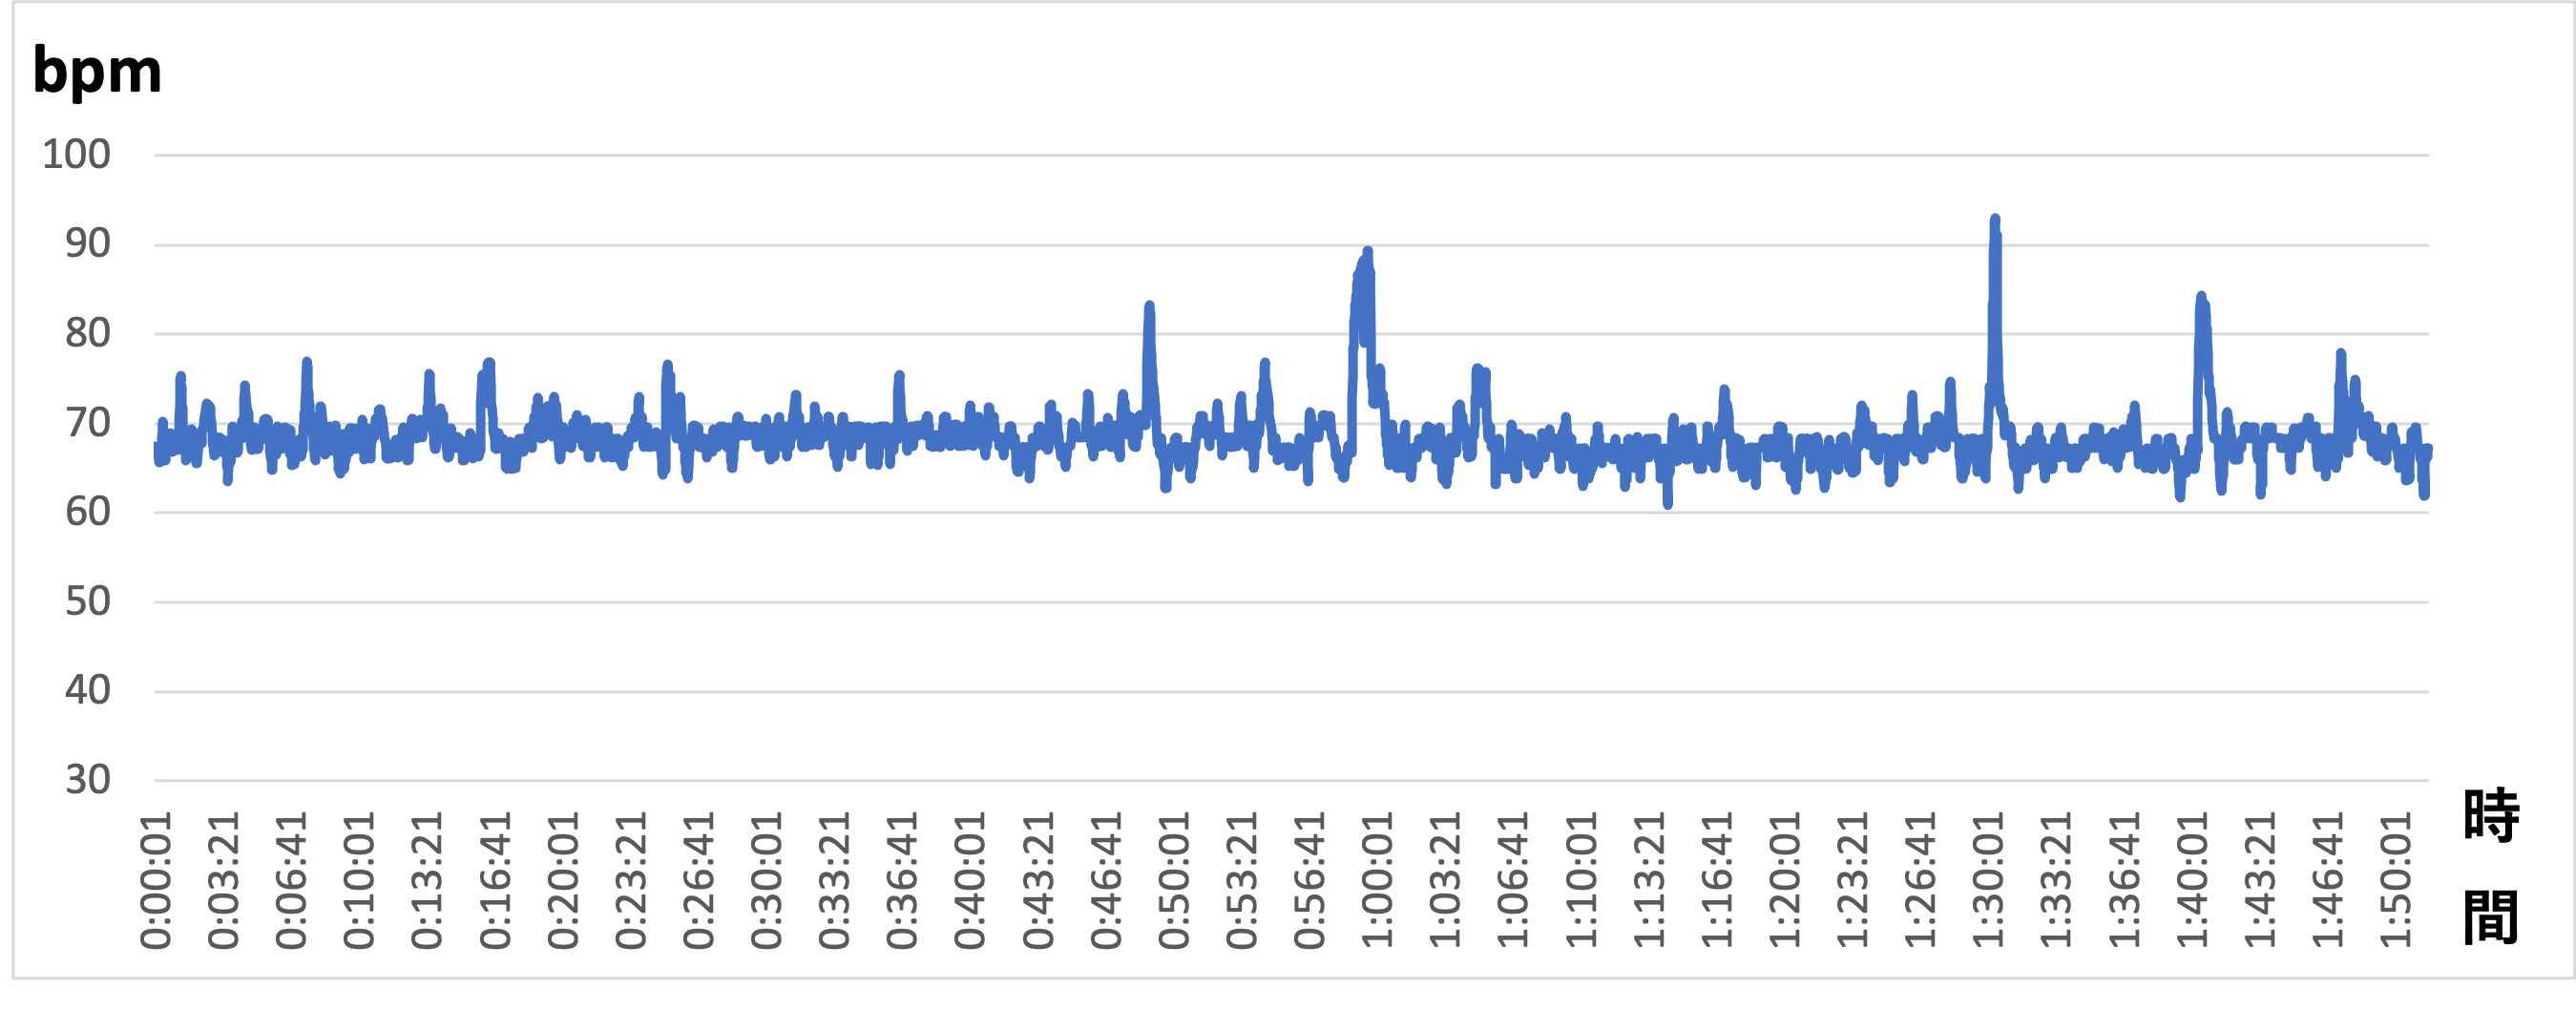
\includegraphics[width=16cm]{images/chapter3/gurafu2.png}
    \caption{キングコングを視聴した時の1人目心拍数のグラフ}
    \label{hitorime}
\end{figure}

\begin{figure}[H]
    \centering
    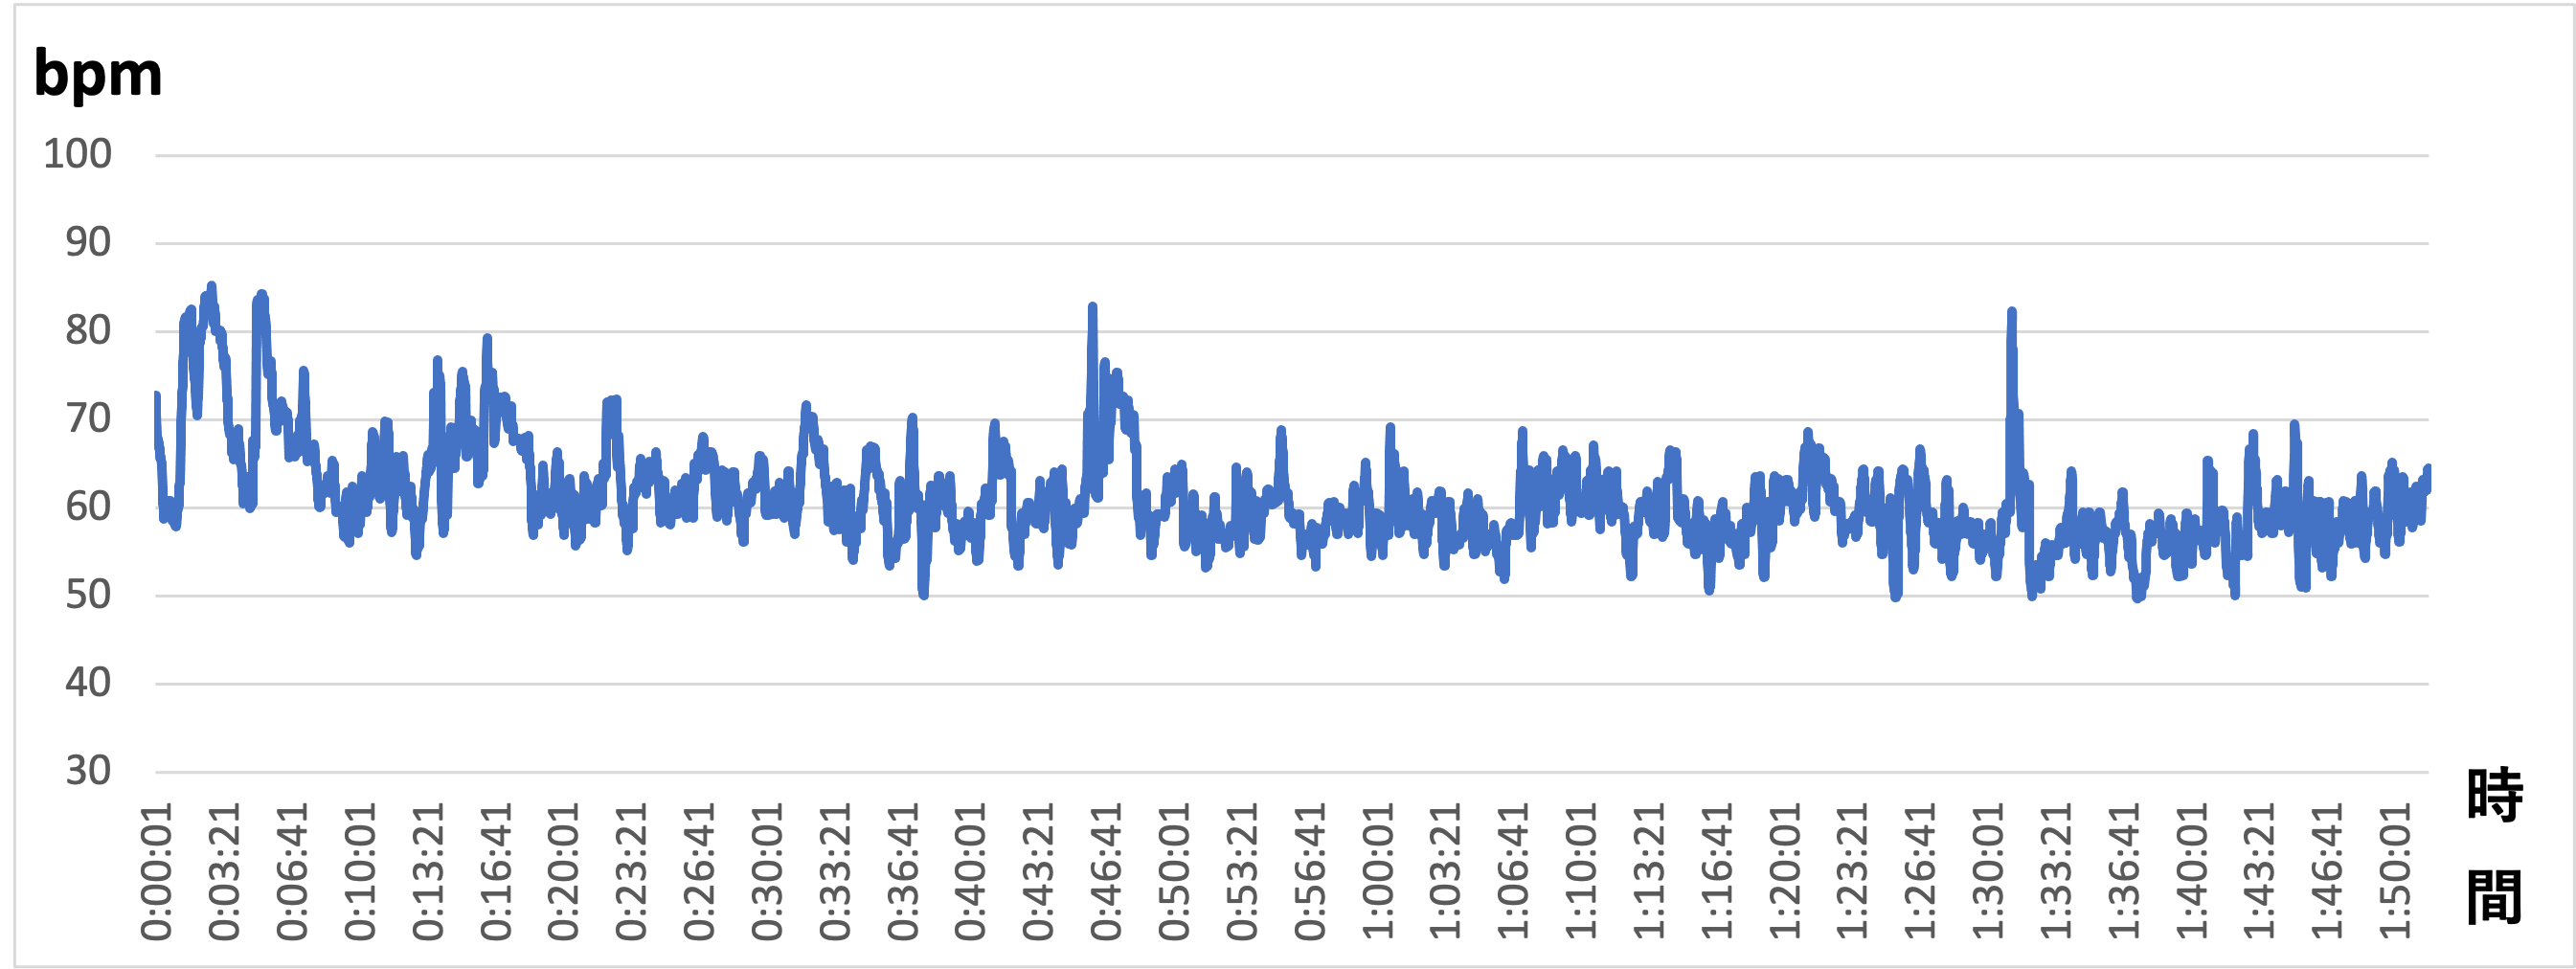
\includegraphics[width=16cm]{images/chapter3/gurafu.png}
    \caption{キングコングを視聴した時の2人目心拍数のグラフ}
    \label{futarime}
\end{figure}

\begin{figure}[H]
    \centering
    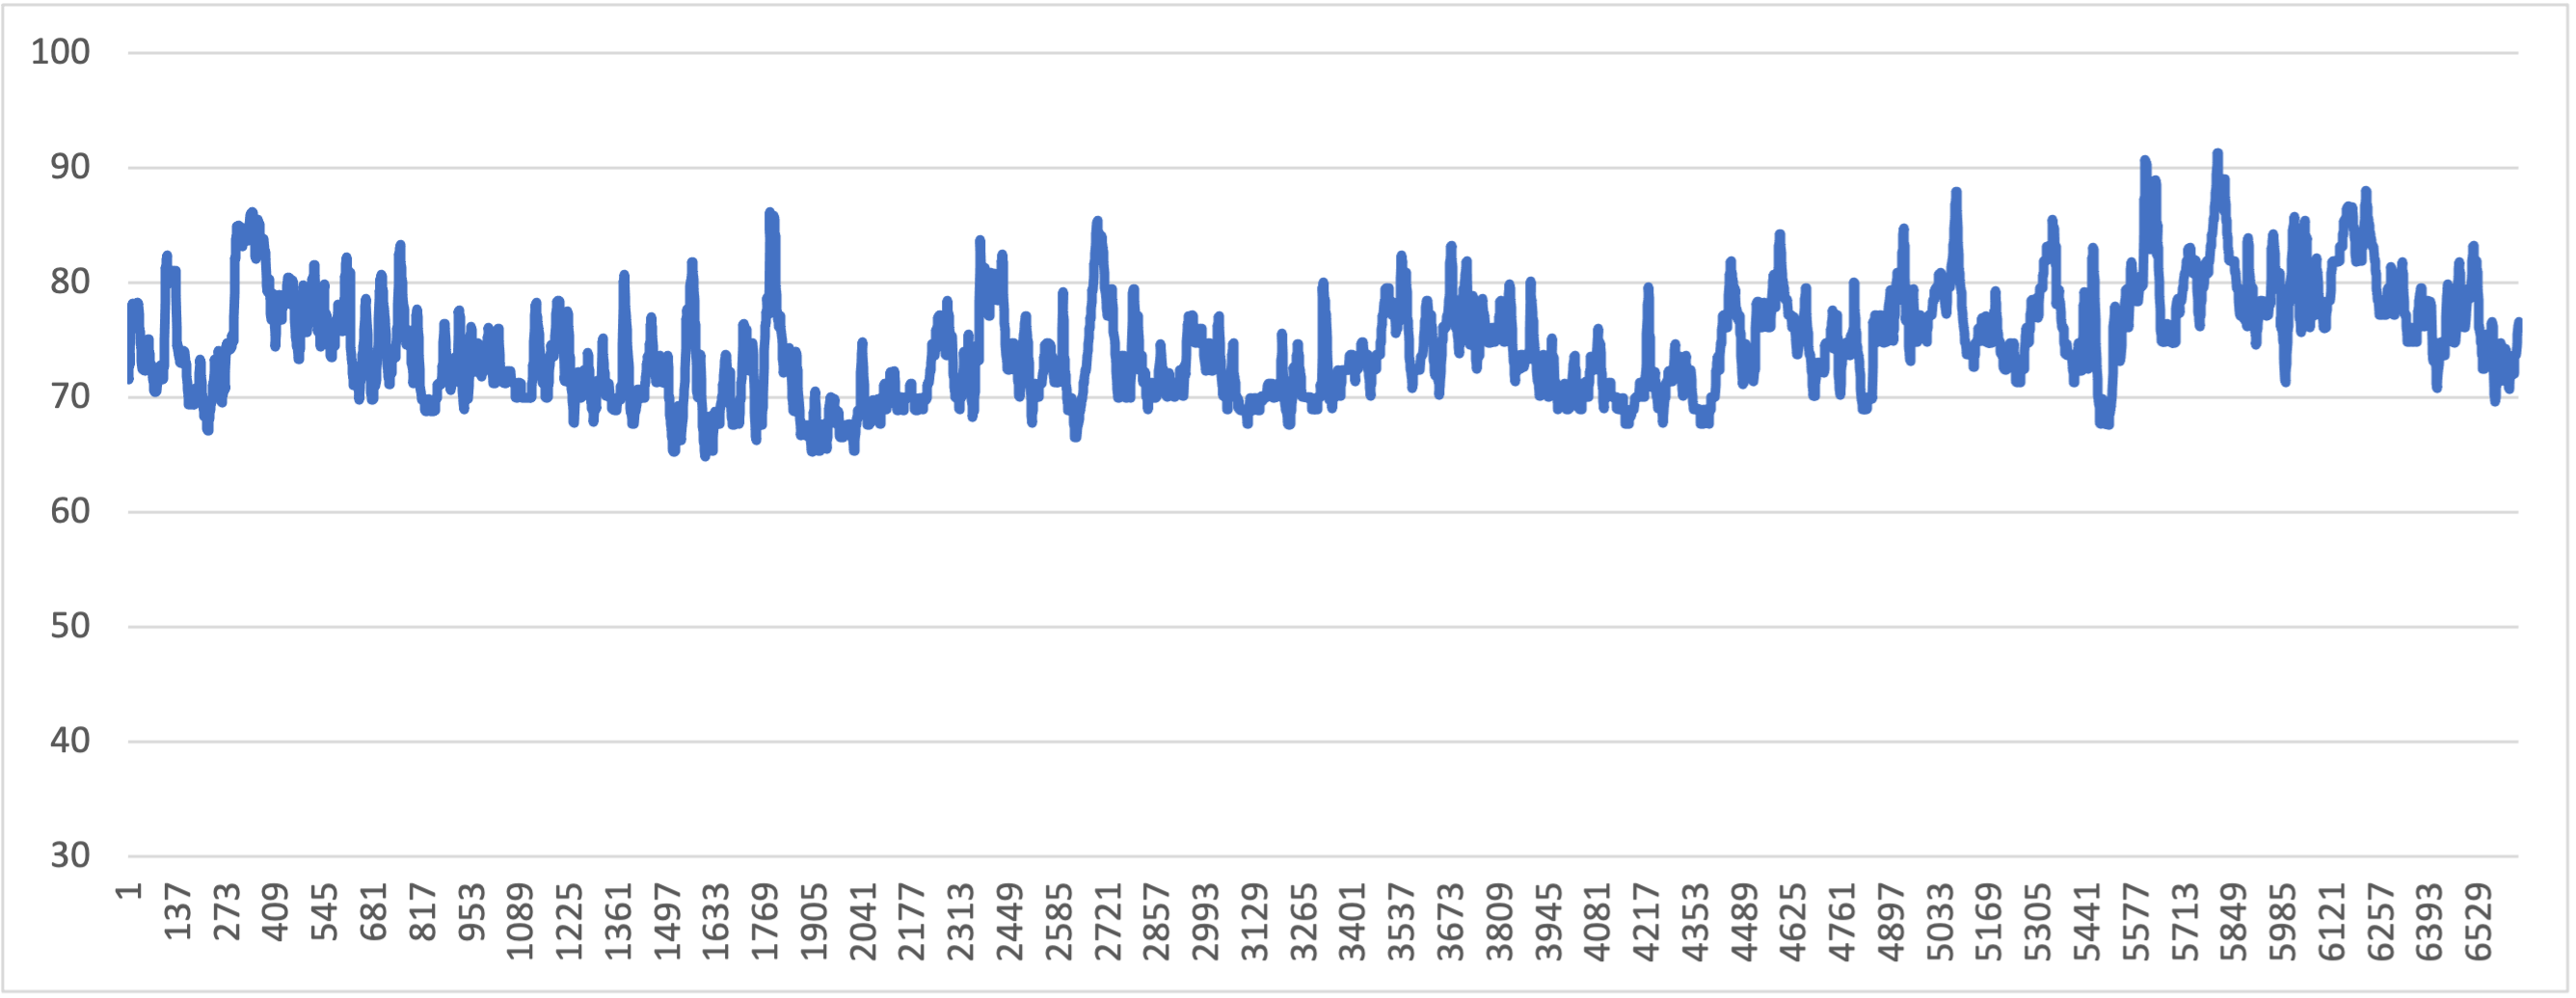
\includegraphics[width=16cm]{images/chapter3/gurafu1.png}
    \caption{キングコングを視聴した時の3人目心拍数のグラフ}
    \label{sannninme}
\end{figure}

\subsection{心拍数上昇箇所の抽出処理}
 収集した心拍データを基に,エフェクト表示に適した形式にするため心拍数が上昇している箇所を抽出するための処理を行う.
収集した心拍数の CSV データをエフェクト表示に適したJSON データにする.
エフェクト表示用に作成したデスクトップアプリの都合上本研究ではJSONデータに変換する.
まず,サーバから心拍数のCSVデータを取得し心拍数が上昇している箇所の抽出を行う.心拍数上昇箇所の抽出処理の方法を図\ref{bpmupp}に示す.
収集した心拍データを観察し,心拍数が上昇している箇所の抜き出し方法を決定した.人により平均の心拍数はさまざまであったため,
心拍数が上昇している箇所を見つけ出すようまず安静時の心拍数を取得する.安静時の心拍数は,映画を視聴する前の1分間動かない状態で心拍数を計測し取得する.
その安静時の平均心拍数からどれだけ心拍数が上昇したかを抽出する.これにより心拍数が高い人も低い人も同じ抽出処理が可能になる.
表\ref{model}に今回作成したモデルの定義を示す.from toの形式で心拍数が閾値を超えていた時間を示す.
時間は映画が始まってからの経過時間でエフェクト表示するため相対時間にした.今回from toの形式にしたのは,
エフェクトを映画画面に重畳する際にエフェクト表示する時間を心拍数が閾値を超えていた時間の範囲で表示できるようにするためである.
effectlevelで表示するエフェクトを決定する.effectlevelは表\ref{effectlevel}のように心拍数を閾値と比較する.閾値は収集した心拍データを基に設定した.
心拍数の上昇具合で表示するエフェクトを変更するため,1から3までのレベル分けをした.
本研究ではエフェクトを3段階にし心拍数のレベルに応じて表示するエフェクトが変更される.安静時の平均心拍数よりも心拍数が16bpm以上高い時をレベル3,
14bmp以上をレベル2,12bpm 以上をレベル1とする.実際に心拍数上昇箇所の抽出処理をした後のデータを図\ref{bpmsyori}に示す.


\begin{figure}[H]
    \centering
    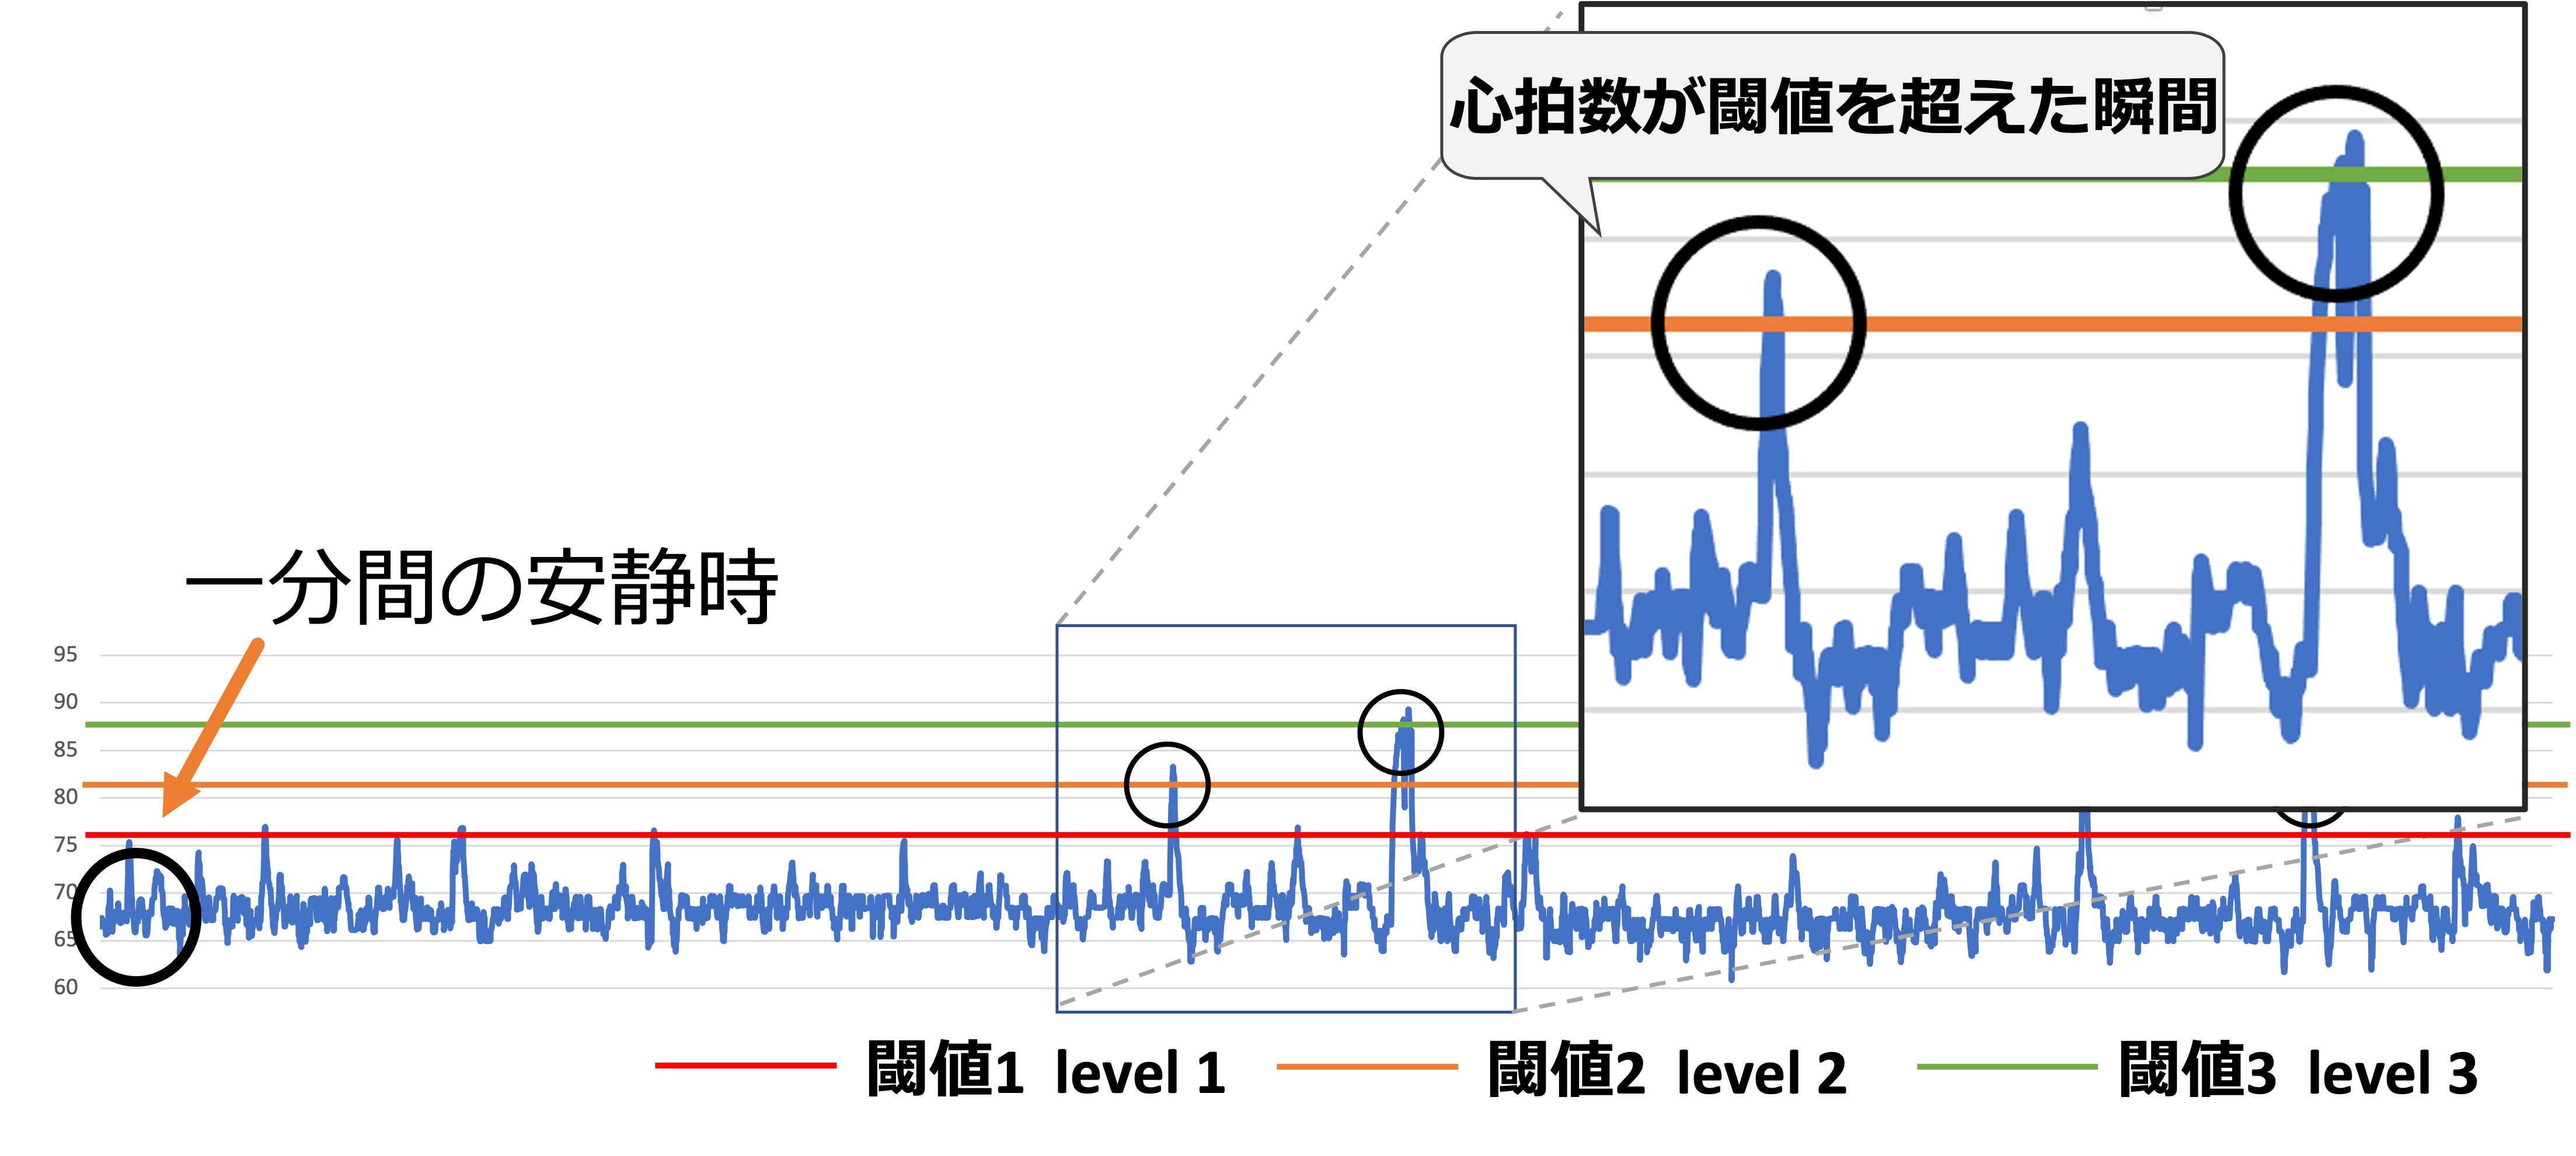
\includegraphics[width=16cm]{images/chapter3/haisyutusyori.png}
    \caption{心拍数上昇箇所の抽出処理}
    \label{bpmupp}
\end{figure}


\begin{table}[htb]
    \begin{center}
        \caption{心拍データのモデルの型定義}
        
        \label{model}
            \begin{tabular}{|c|c|c|} \hline
            	プロパティ & 型 & 説明  \\ \hline \hline
                from & float & 心拍数が閾値を超えた時間 \\ \hline
                to & float & 心拍数が閾値を下回った時間 \\ \hline
                effectlevel & int & 表示するエフェクトのレベル \\ \hline
            \end{tabular}
    \end{center}
\end{table}


\begin{table}[htb]
    \begin{center}
        \caption{閾値設定}
        
        \label{effectlevel}
            \begin{tabular}{|c|c|c|c|} \hline 
            	effectlevel & 1 & 2 & 3  \\ \hline 
                閾値 & 16bpm以上 & 14bpm以上 & 12bpm以上 \\ \hline
            \end{tabular}
    \end{center}
\end{table}



\begin{figure}[H]
    \centering
    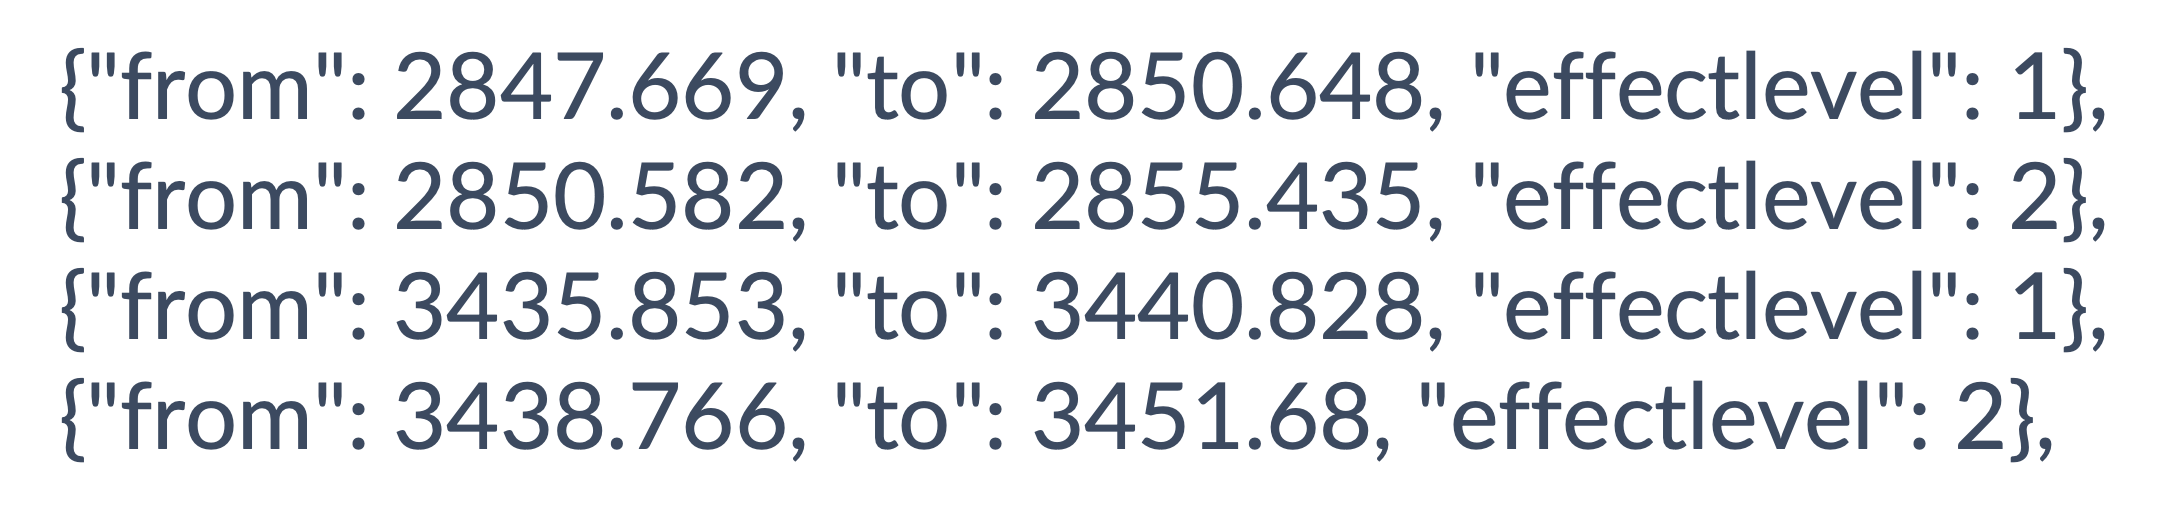
\includegraphics[width=16cm]{images/chapter3/level.png}
    \caption{心拍数上昇箇所の抽出処理をした結果}
    \label{bpmsyori}
\end{figure}


 エフェクト表示に適した形式にするため、心拍数上昇箇所の抽出処理したJSONデータを一つのJSONデータにまとめる.
JSONデータの概要を図\ref{gaiyou}に示す.これにより一つのコンテンツに一個のJSONデータが作られる.このデータを使いエフェクトを映画画面に重畳する.

\begin{figure}[H]
    \centering
    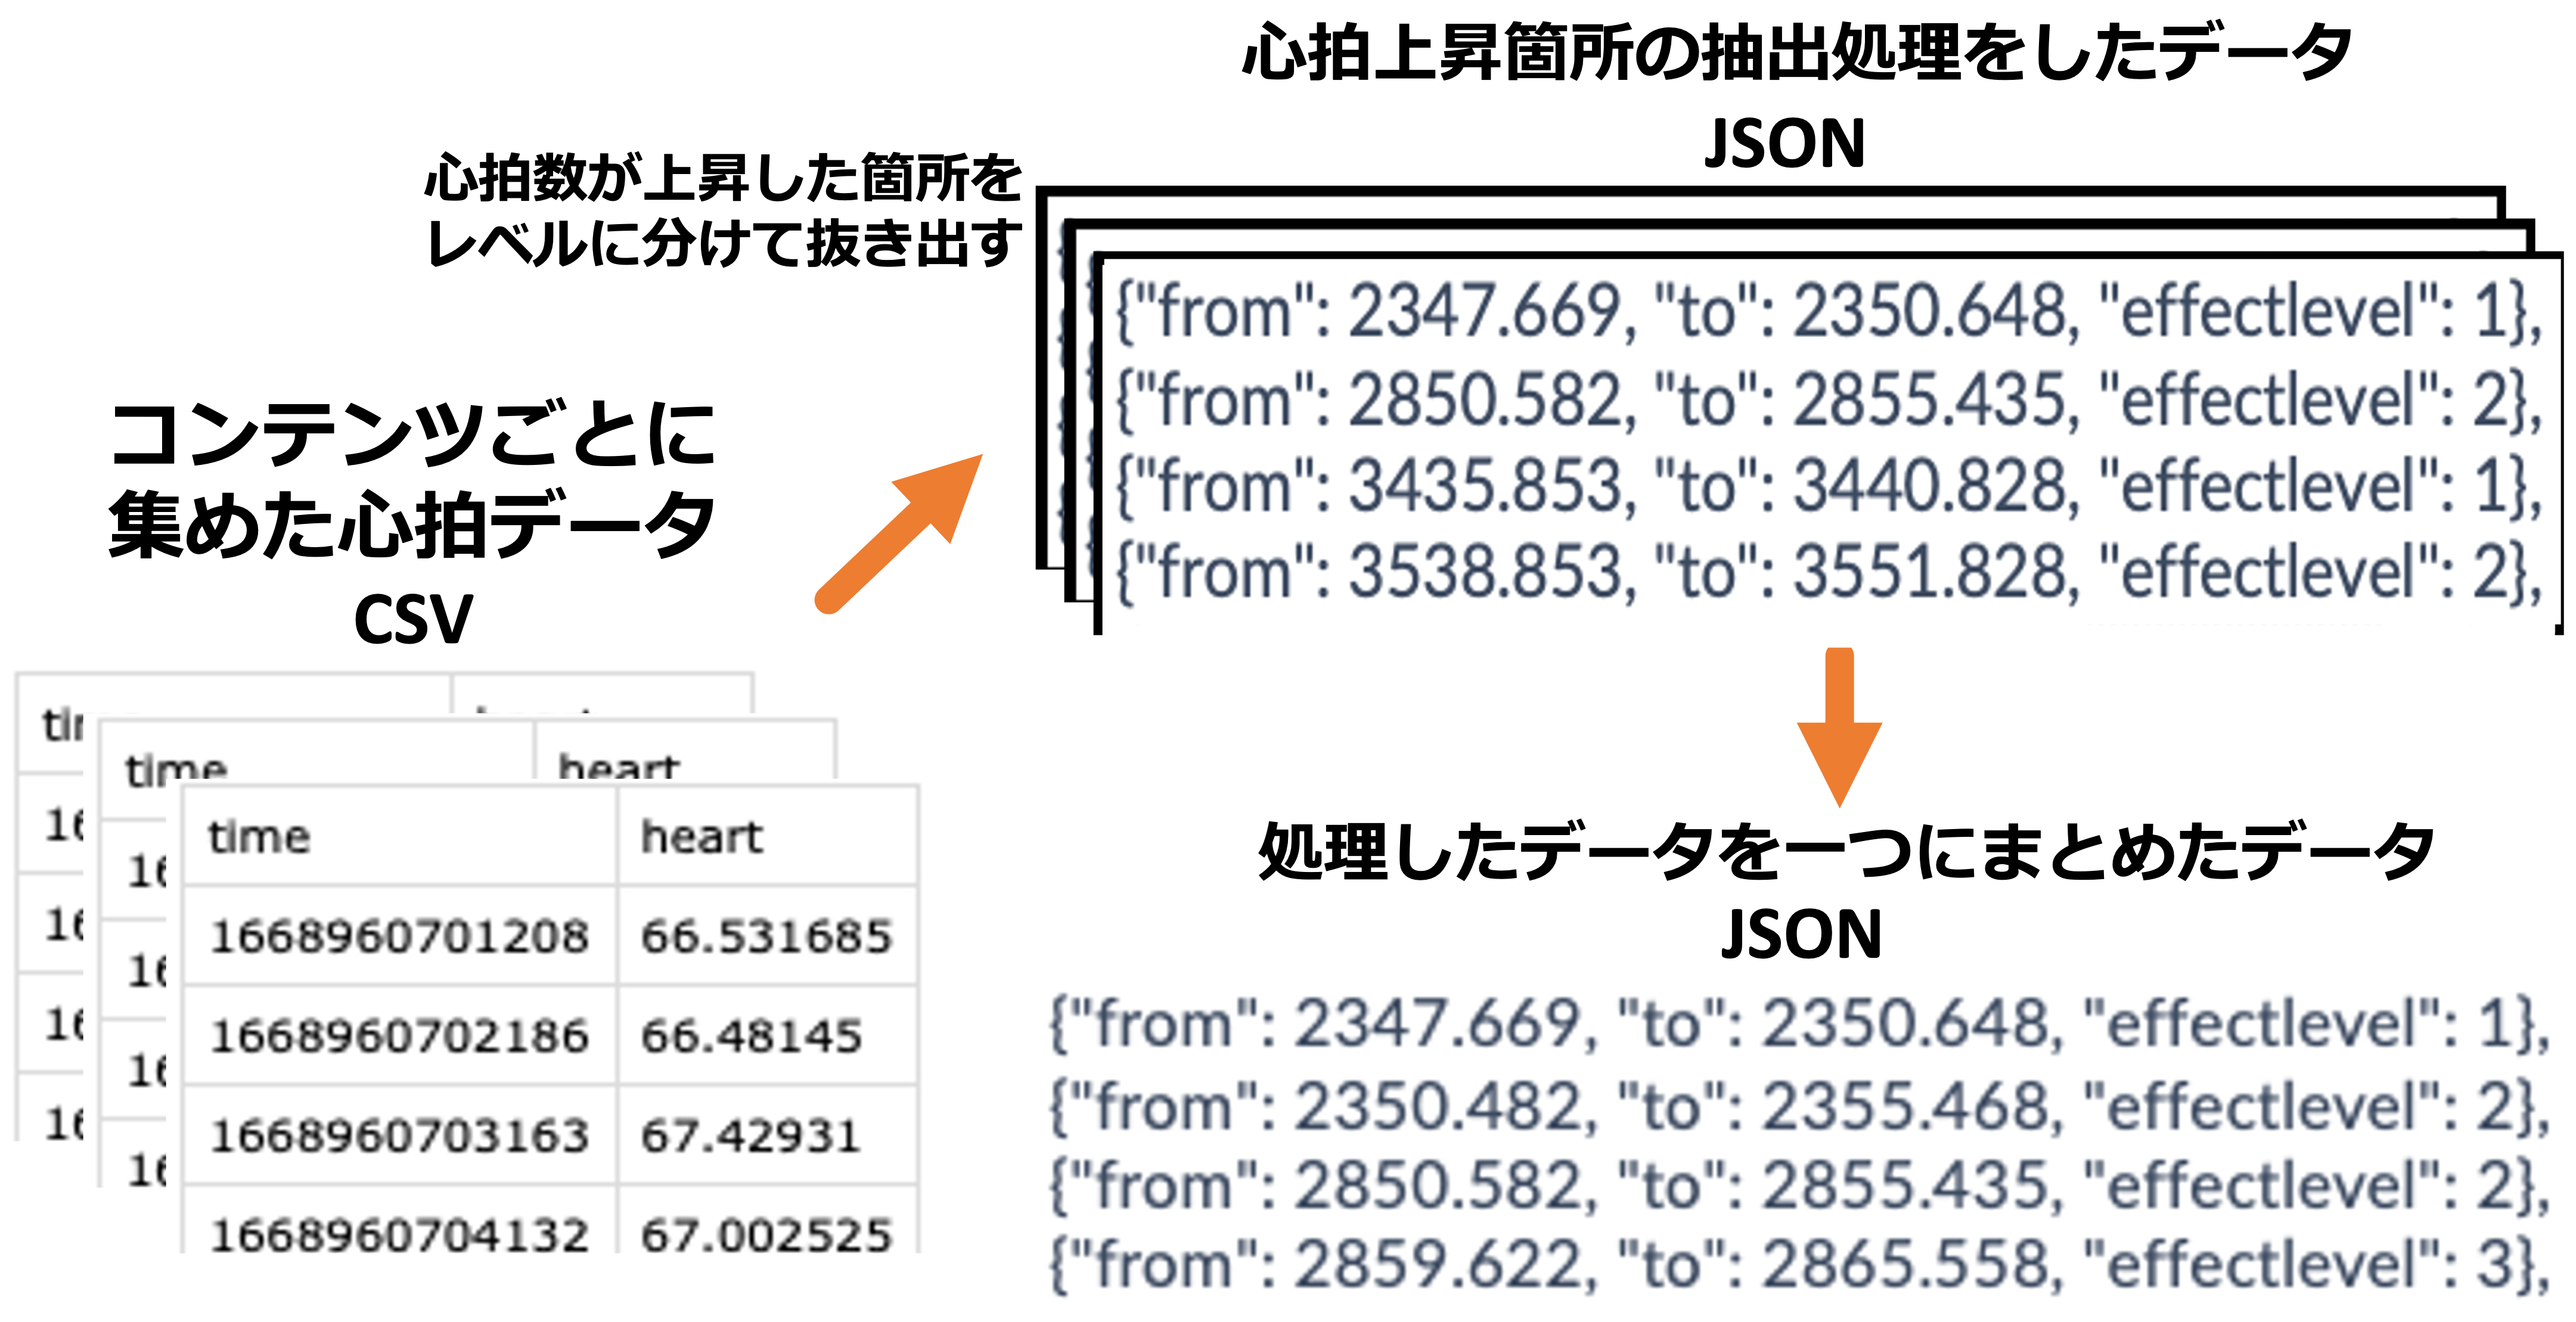
\includegraphics[width=16cm]{images/chapter3/system.png}
    \caption{心拍データの概要図}
    \label{gaiyou}
\end{figure}







\section{生体データを用いたコンテンツへの重畳提示システム}
\subsection{重畳表示の概要}
目的として、自宅でPCを使用し離れている場所でも動画視聴をしている中で盛り上がっているシーンをエフェクトとして共有でき,新しい映像効果を与えるコンテンツを開発する.


\subsection{システム構成}
システム構成は、処理したデータをElectronのデータファイルに転送し、サーバーでレベルごとに分けられた結果を基にElectronでエフェクトを重畳提示する。
Electron(エレクトロン)とは、ウェブ技術でデスクトップアプリケーションを作成できるテクノロジーである。HTMLとCSS、JavaScriptを使用し開発、WindowsとmacOSの両OSのアプリケーションを1つのコードから作ることができ、ウェブコンテンツをそのままアプリケーションとして動かすことができ、デスクトップアプリケーションとしてブラウザだけで実現できない機能の組み込みが出来るため使用した。
Electronを使用する目的として、コンテンツ共有を複数人で行うことができ個人で重畳提示手法を選択可能にするためである。複数人でコンテンツ共有とは、視聴している動画に対して取得しているユーザの心拍数を基にエフェクト重畳を行うためである。個人で重畳提示手法を選択可能とは、視聴している動画のジャンルごとにエフェクトの種類を個人で選択可能にし、新しい映像効果を与える。
エフェクト表示するためのサーバーとのデータ連携については、サーバーからレベルごとに分けたデータを転送し、Electronで受信したデータを基にレベルごとにエフェクト提示を行う。本研究ではリアルタイムでデータ送信が出来なかった為、手動でのデータ転送を行なっている。レベルごとにエフェクト提示は、リアルタイムでデータ転送ができず、エフェクト制作の際にAfterEffectsを使用した為レベル分けを行なった。AfterEffectsの使用では透過tiff書き出しを行うことで,エフェクト提示の際に透過の範囲が決めやすく、エフェクト修正を即時変更可能であるため。そのため、エフェクトをダイナミックに生成できず、細かな心拍数変化の表示ができていない。
エフェクト提示方法として、Electronを起動,視聴する画面に重畳を行い、視聴する動画を選択、提示するエフェクトを選択、Playをクリックすることでエフェクト重畳が開始する。
その例を図に示す.

\begin{figure}[H]
    \centering
    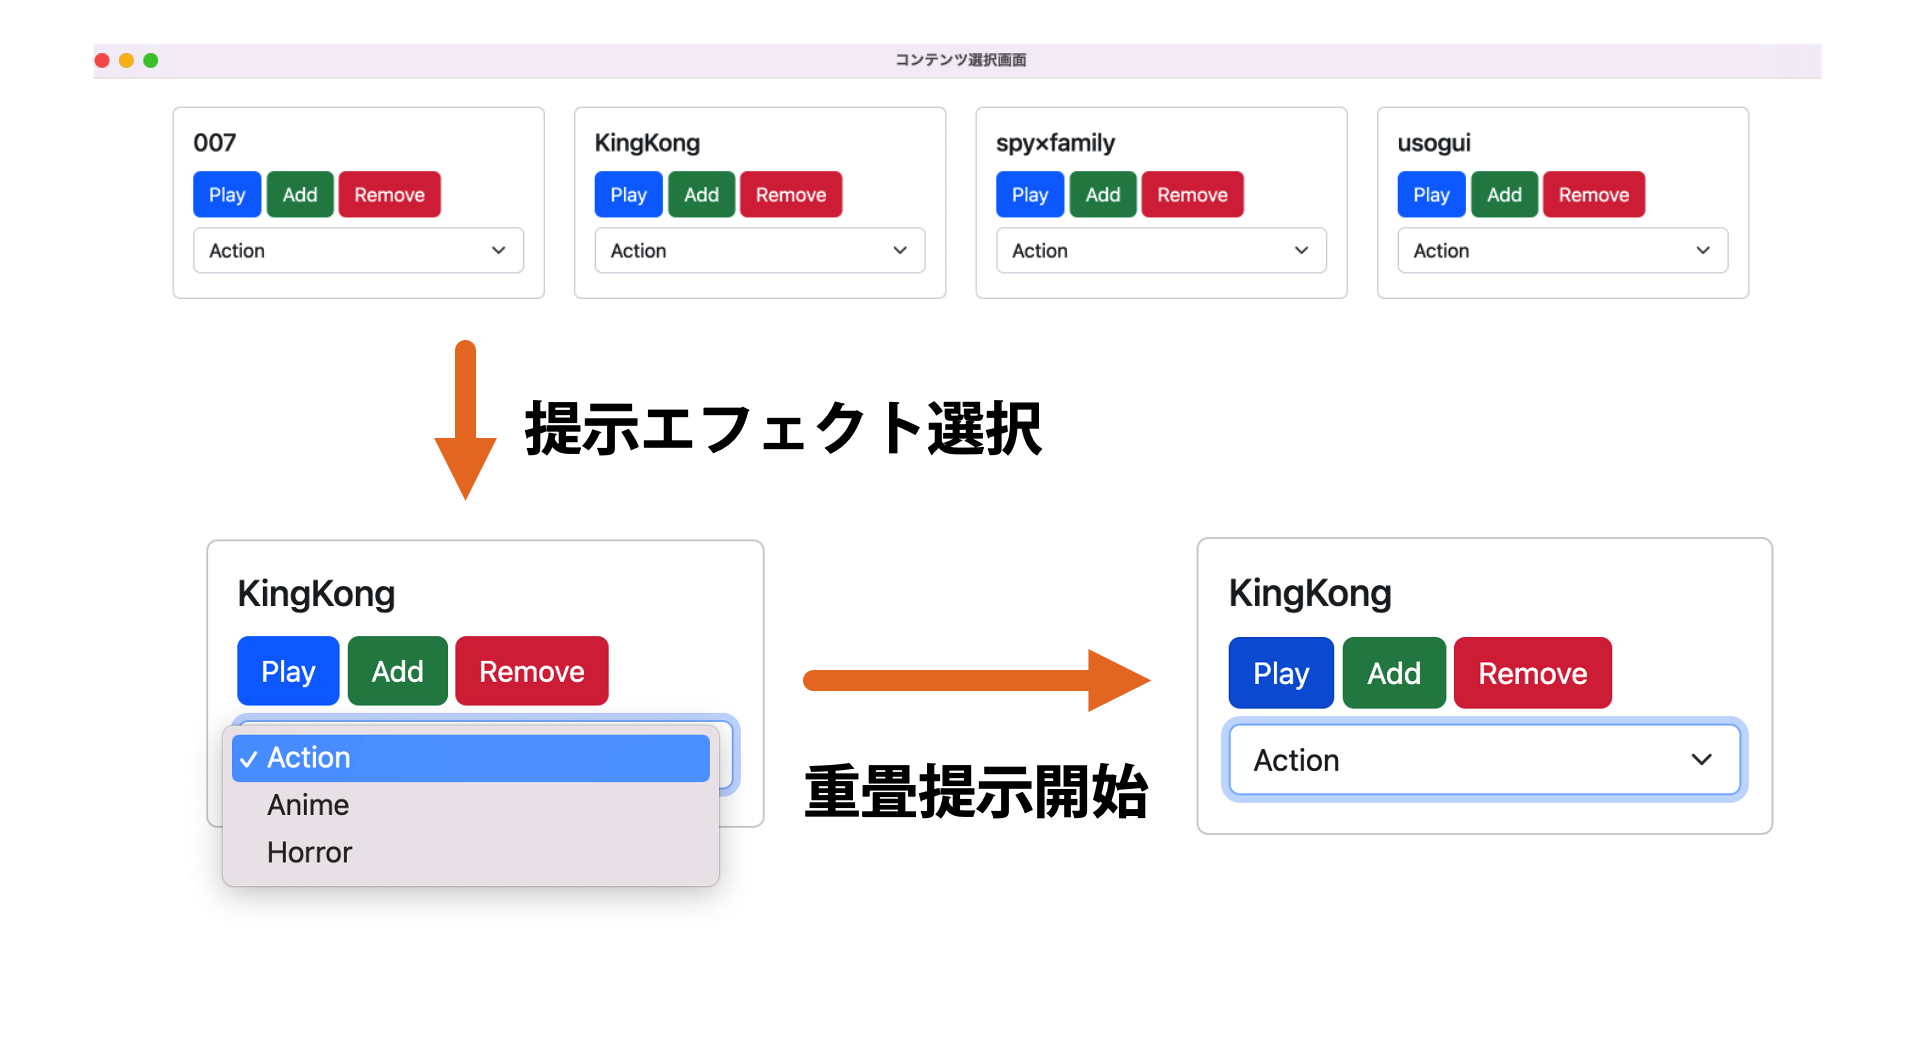
\includegraphics[width=17cm]{images/chapter3/efect_setumei.png}
    \caption{Electron動作画面(エフェクト提示選択)}
\end{figure}

\subsection{エフェクトの提示}
エフェクトの提示として,表示するエフェクトを3種類に分け,1種類に2つのエフェクトを制作した.エフェクトを種類別に分けたのは,視聴する映画のジャンルを3種類(Action,Anime,Horror)に分け新しい視聴効果を引き出すためである.
エフェクトの目的として,Actionは迫力/緊迫感を与える,Animeはより面白さを与える,Horrorは恐怖感を軽減させるとして制作した.エフェクト提示の実装画面を図\ref{efectteiji}に示す.
Actionのエフェクトは,迫力/緊迫感を与える目的のためノイズの赤色を画面の両淵に配置し,視聴に影響が出ないようにした.制作方法としてAfteEffectsを使用し,フラクタルノイズ効果/色かぶり補正を使用した.フラクタルノイズ効果はコントラスト60,明るさ0.0,複雑度6.0,展開1×+190.0,不透明度100.色かぶり補正はブラックをマップのカラーを黒,ホワイトをマップのカラーを赤にした.エフェクトレベルが上がることでコントラストを80に上げて制作した.評価実験を繰り返す中で,画面全体に赤色と黒色のぼかしエフェクトを重畳することで映像視聴に影響が出てしまい,エフェクトに目が注視してしまい映画視聴がしずらい意見があったため画面の両端にエフェクトを配置し黒色のの歌詞をなくす修正をおこなった.図\ref{actionbefore}にエフェクト修正前と修正後を示す.Animeのエフェクトは,より面白さを与える目的のため漫画などで使用される効果線を画面全体に配置し視聴の邪魔にならずエフェクト効果を感じられるようにした..制作方法としてIllastratorを使用し,ペンツールで塗りを白,線をなしにした.エフェクトレベルが上がることで白色の効果線の数を増やし,白の太さを太く,黒の効果線を増やすことでエフェクト効果を感じられるようにした.Horrorのエフェクトは,恐怖感を軽減させる目的のため画面全体に白のノイズをかぶせることで映像を見やすくするようにした.制作方法としてAfteEffectsを使用し,フラクタルノイズ効果/色かぶり補正を使用した.フラクタルノイズ効果はコントラスト50,明るさ0.0,複雑度3.0,展開1×+100.0,不透明度100.色かぶり補正はブラックをマップのカラーをなし,ホワイトをマップのカラーを白にした.エフェクトレベルが上がることでコントラストを70に上げて制作した.評価実験を繰り返す中で,画面全体に灰色のぼかしエフェクトを重畳することで映像視聴に影響が出てしまい,映像自体が見えなくなってしまう意見があったため画面中心を白くし周りを薄い白色でぼかす修正をおこなった.図\ref{horrorbefore}にエフェクト修正前と修正後を示す.

\begin{figure}[H]
    \centering
    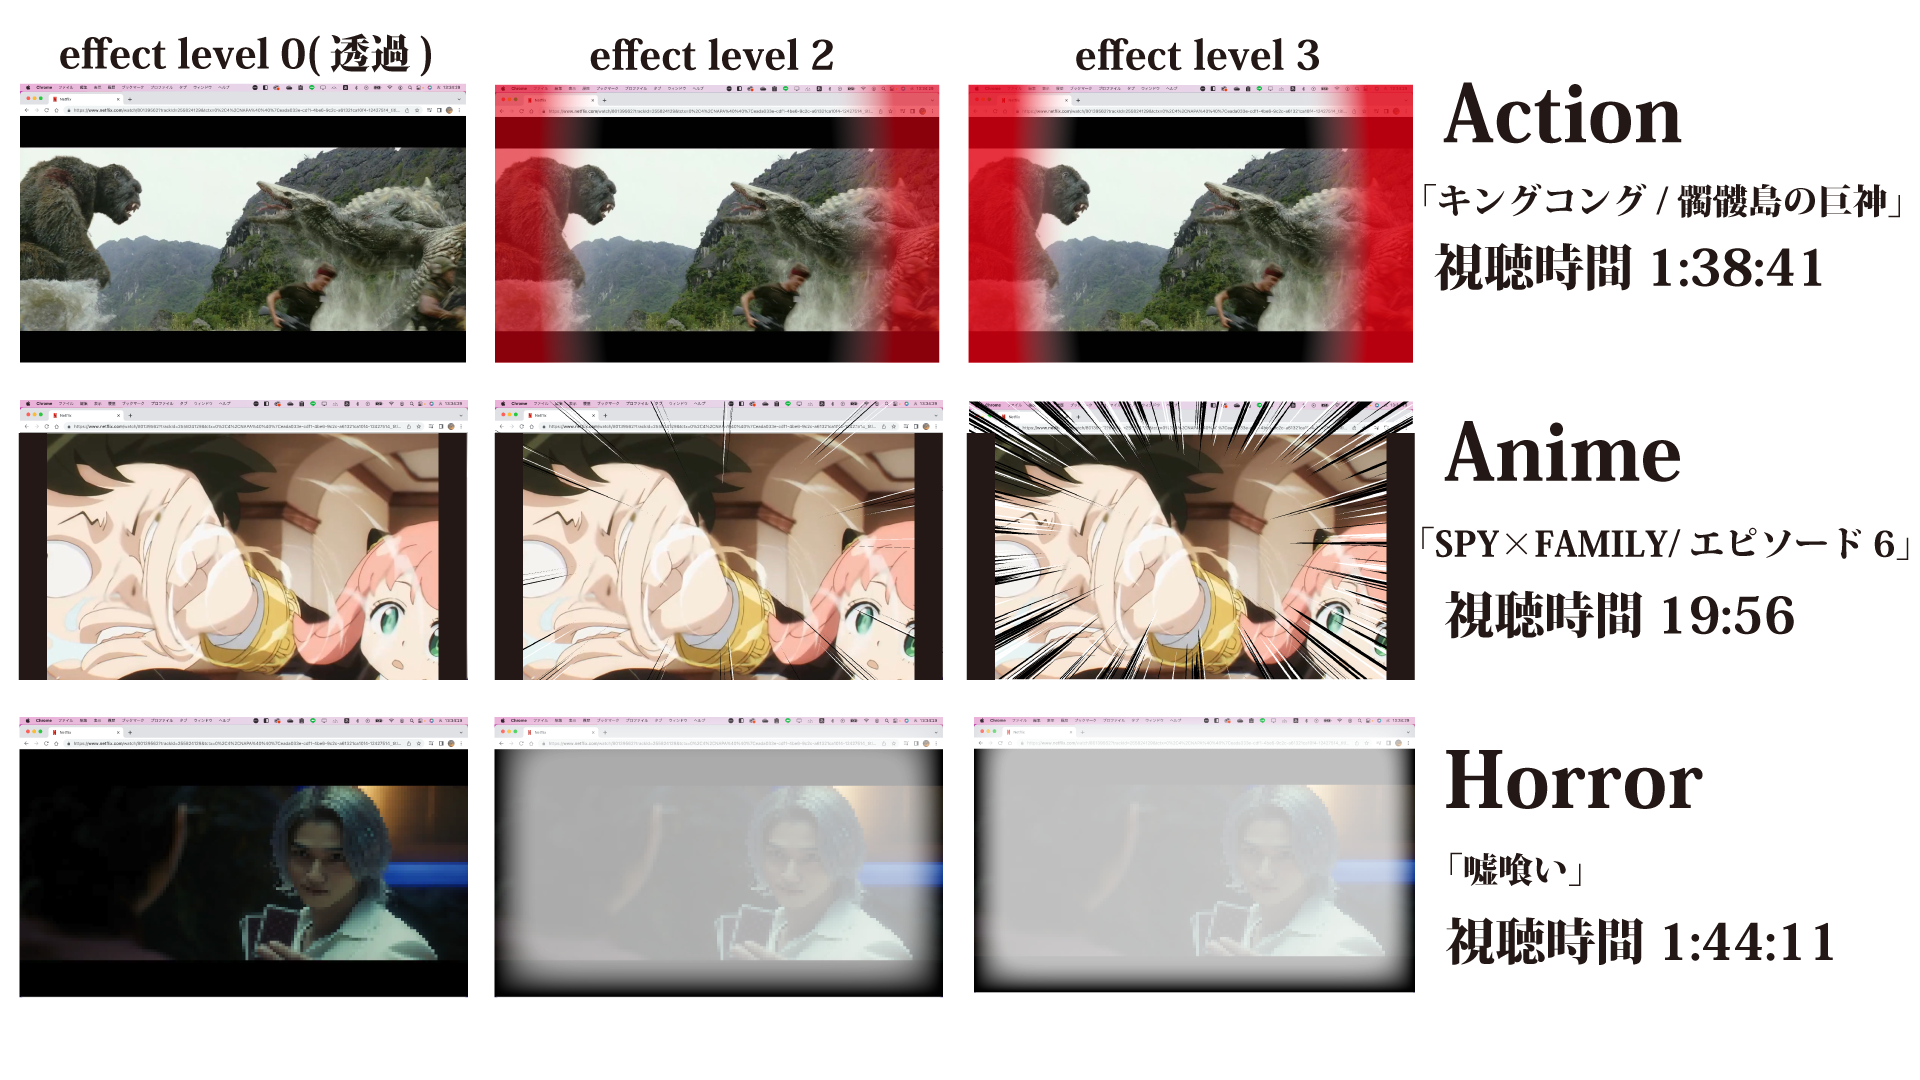
\includegraphics[width=16cm]{images/chapter3/efects.jpg}
    \caption{エフェクト提示画面}
    \label{efectteiji}
\end{figure}

\begin{figure}[H]
    \centering
    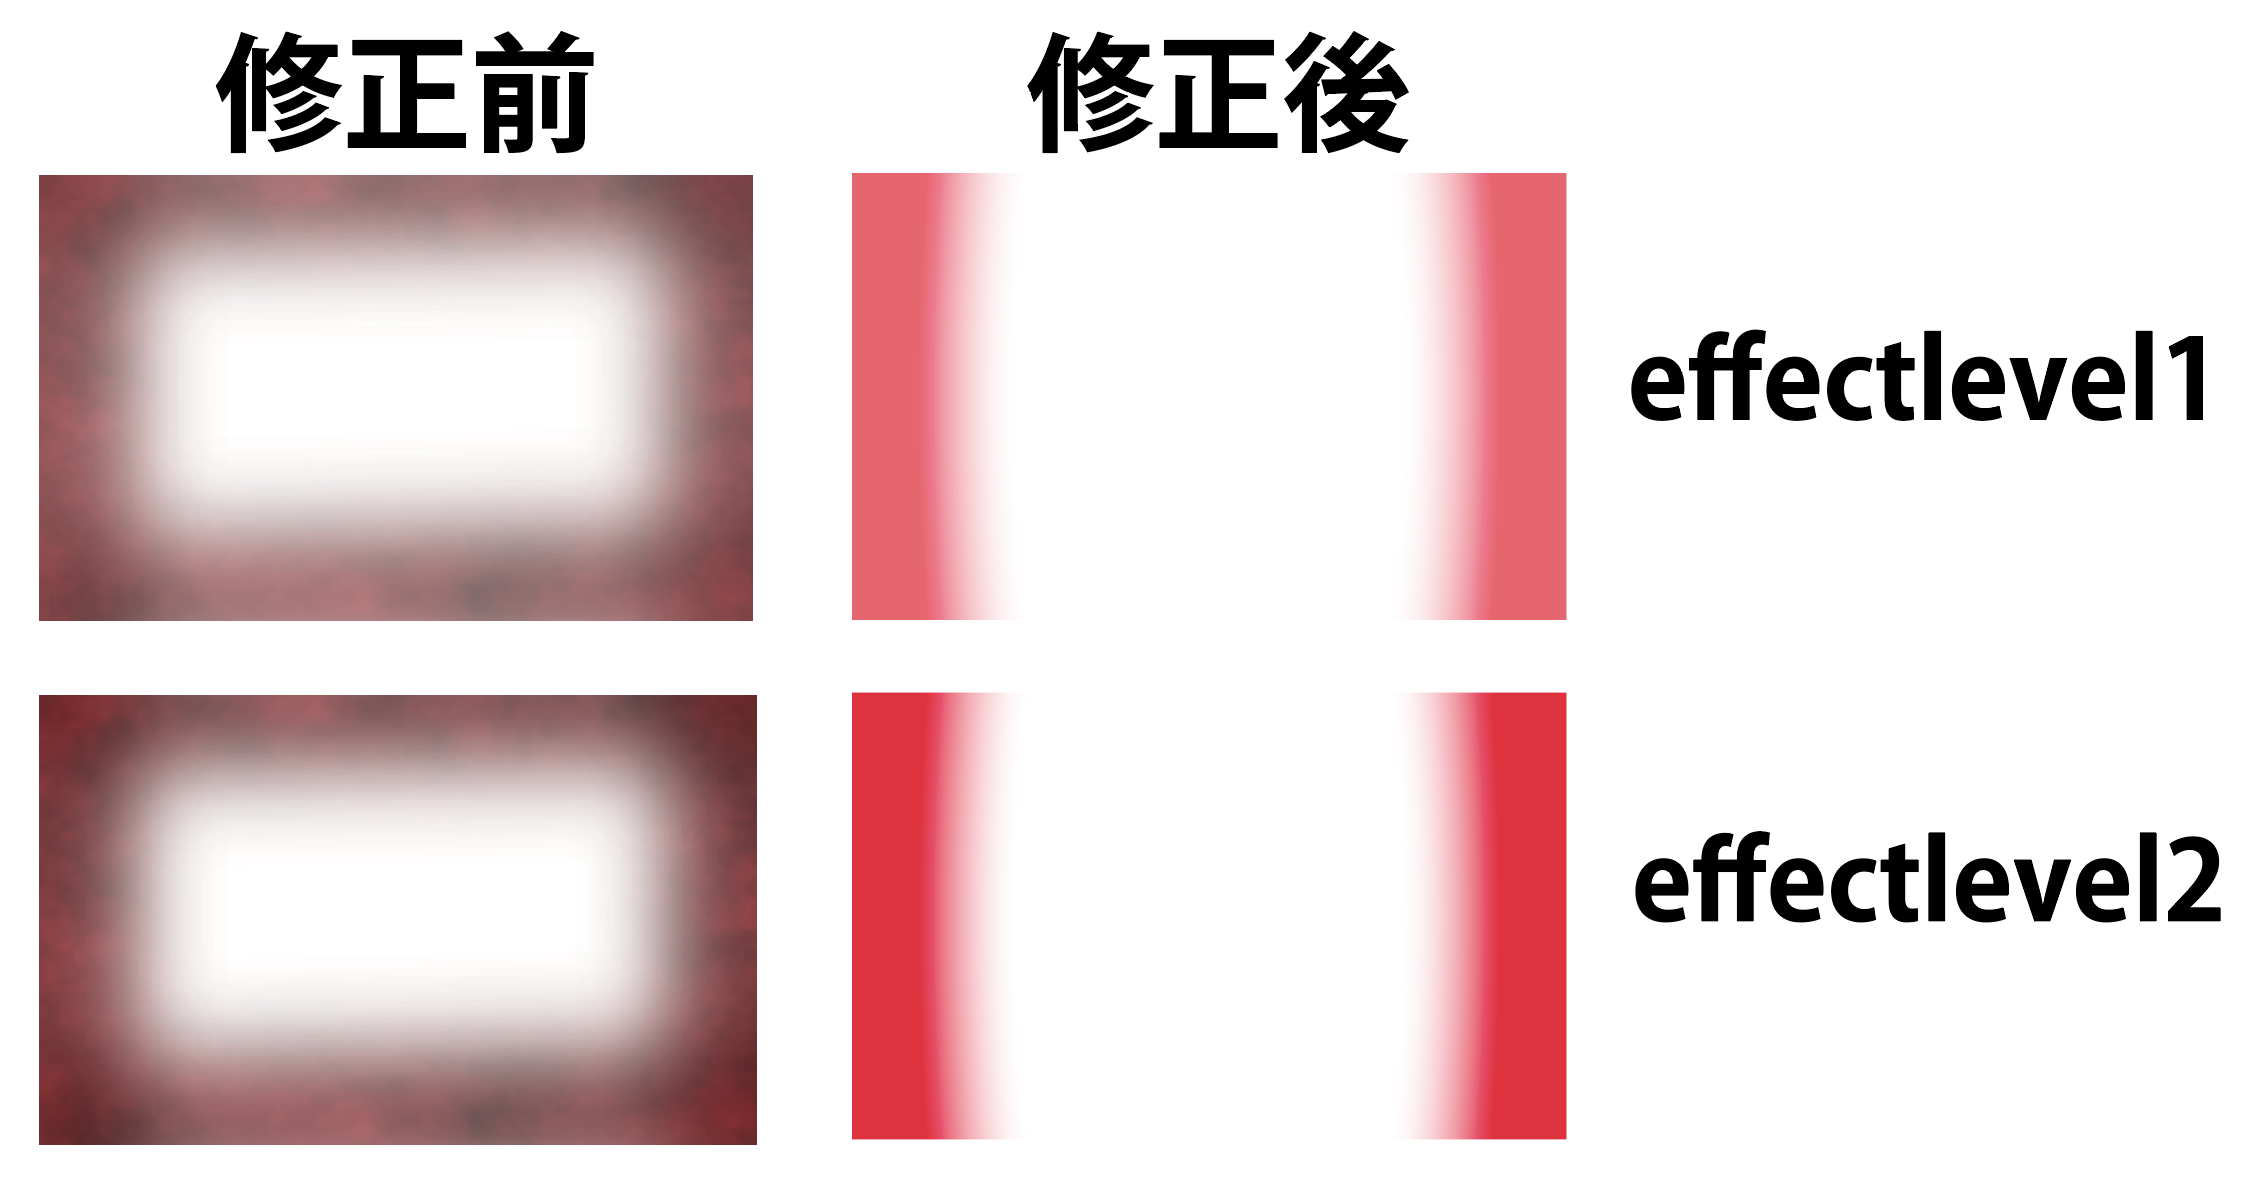
\includegraphics[width=16cm]{images/chapter3/actionberore.jpg}
    \caption{Actionエフェクトの修正}
    \label{actionbefore}
\end{figure}

\begin{figure}[H]
    \centering
    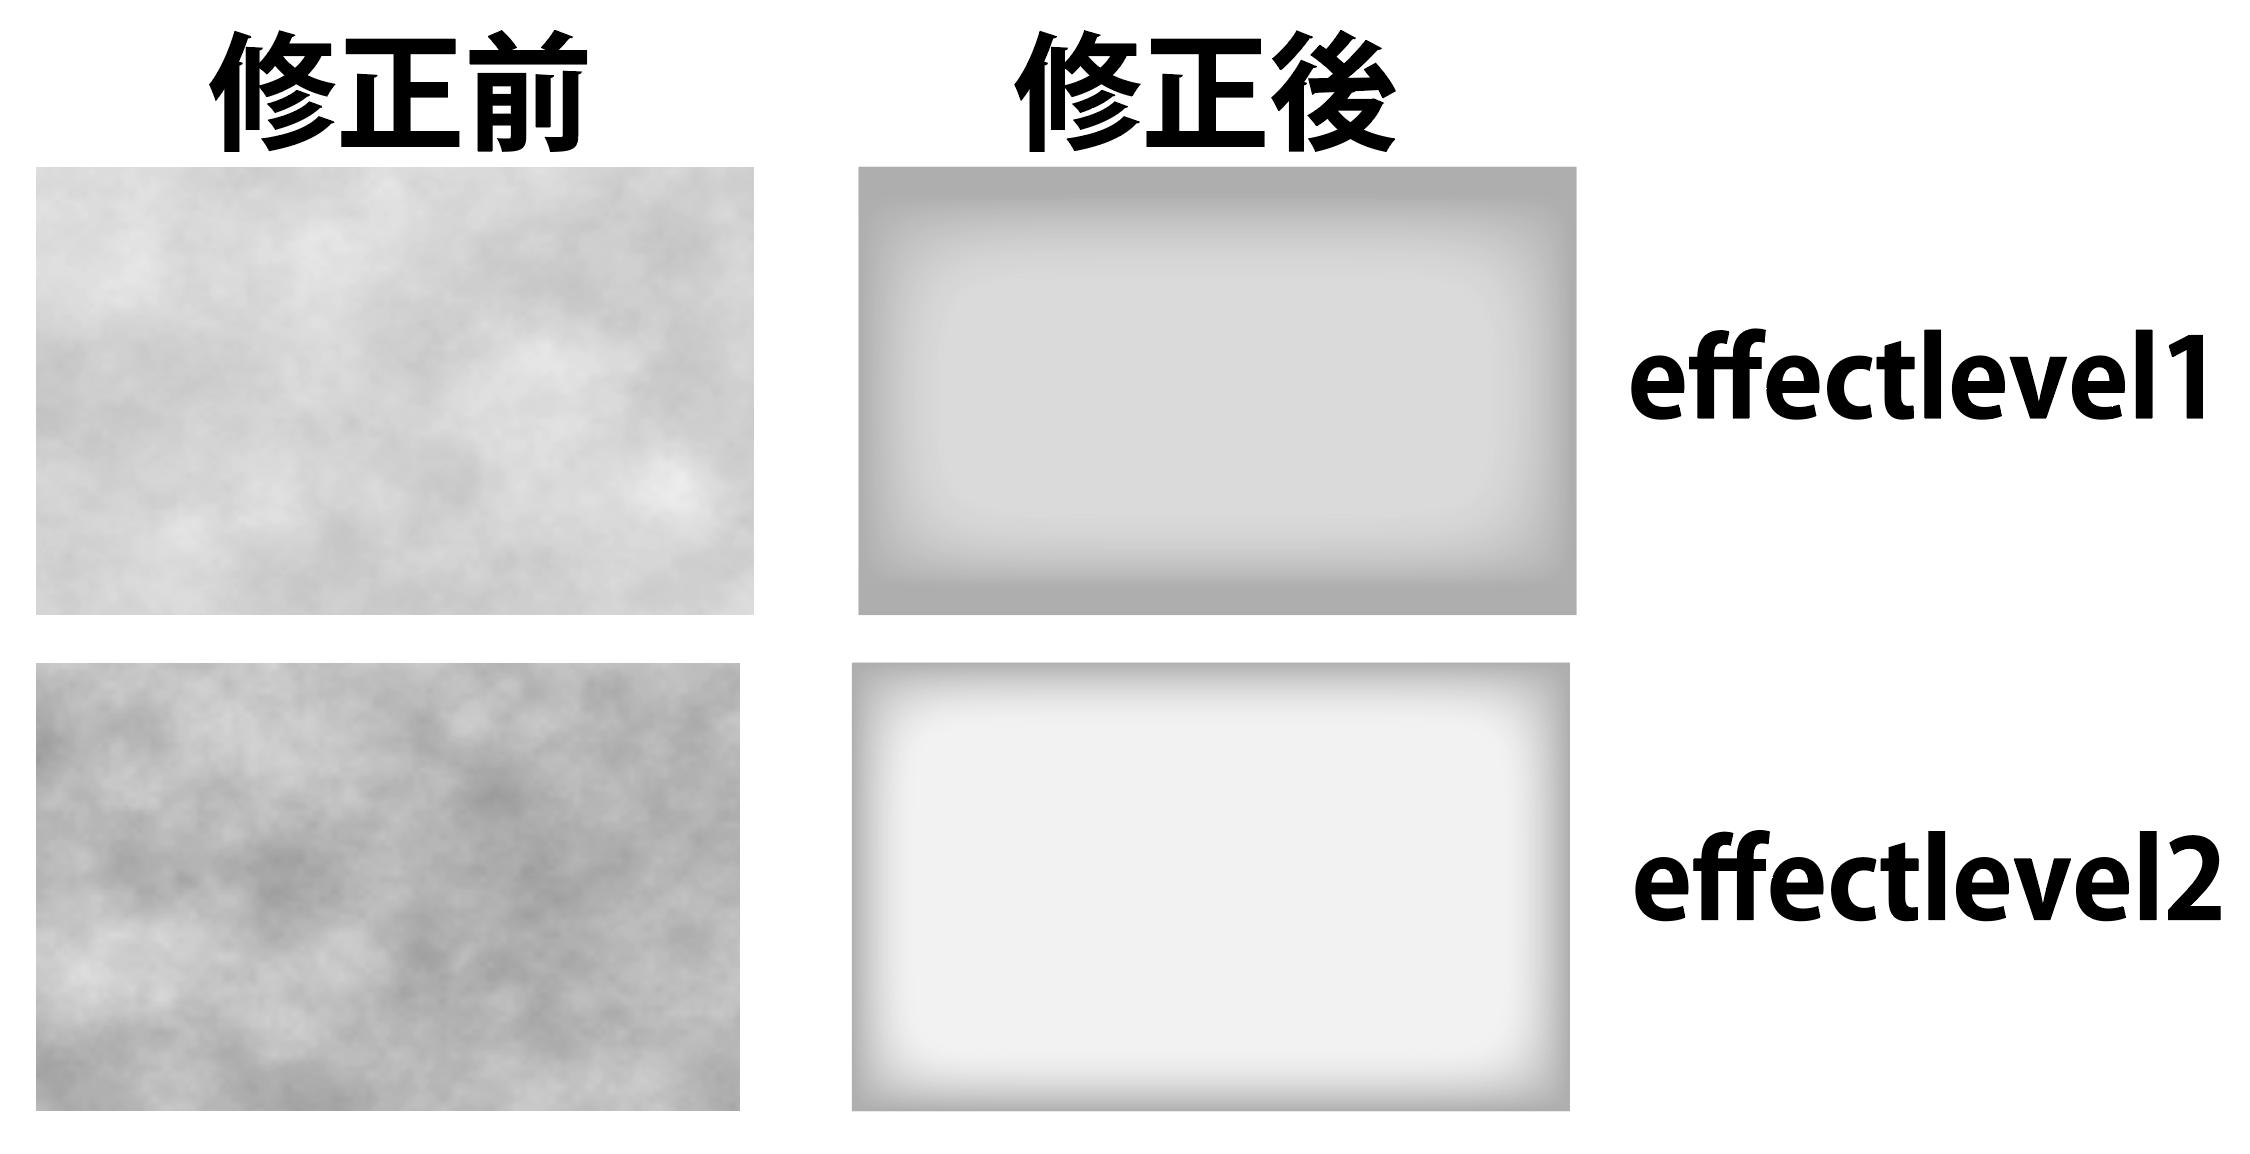
\includegraphics[width=16cm]{images/chapter3/horrorbefore.jpg}
    \caption{Horrorエフェクトの修正}
    \label{horrorbefore}
\end{figure}